% Allow relative paths in included subfiles that are compiled separately
% See https://tex.stackexchange.com/questions/153312/

\providecommand{\main}{..}
\documentclass[\main/thesis.tex]{subfiles}
\externaldocument{}

% \iffalse
% - Capturing and playing sound, digitally
% - Representation (single frame vs multi(spectrum))
% - Creating sound
%     - Sound can be created functionally
%     - sound can be created piece by piece 
% - a quick history/summary of computer music technology (the parts of it that are relevant to our project)
%     - Define vsts, synth parameters, filters, eqs since some they're involved in some of the previous works.
% - Past work involving heuristic search and digital synths
% - Past work involving generative neural nets
% - Our work and how it's different or extends past work 
%     - How it can be replicated
% \fi

% todos:
% properly use amplitude and magnitude and power
% haven't described timbre 
% make reconstruction wave include multiple waveforms and how they go missing if sampling rate too slow
% haven't described nyquist frequency
    
\begin{document}

\chapter{Background and Related Work}
\label{section:background}
This chapter aims to provide a background for the subsequent chapters via a quick overview of four important topics:\\ 
\begin{enumerate}[label=(\roman*)]
\item Digital sound, its features and concepts that have been fundamental to our work.
\item A quick overview of common digital synthesis techniques.
\item Discussion on the applications of artificial neural networks (ANNs) for feature extraction and sound production. Although similar results can be yielded from either approach, we distinguish ANN based techniques from tradition digital signal processing (DSP).
\item Related works and their relative similarities and distinctions.
\end{enumerate}
\section{Digital Audio: Sound from Numbers}
Sound is the result of a series of physical events. Most of what we hear is the product of physical disturbances, causing vibrations in our mutually shared, immersive mediums. Sound waves carry these vibrations through air as part of an expanding, spherical wave front; Exponentially losing intensity as they travel away from the source~\cite{cook1999chap4}. 
\\\\

% [graph describing wave amplitude, phase and frequency here]
\\\\
A sound wave can be viewed as the result of a function which governs amplitude through time, where time and amplitude exist in continuous dimensions. Waves can be approximated via a series of samples, associating time steps to a discrete range of amplitude values. 
Given a wave generation method, computers can make sound by sending a series of discrete values to a digital-to-analogue chip, which in turn can
create vibrations within a speaker.  \textit{Digital synthesis} of audio is the process of creating these discrete values. 
\\

\subsection{Sampling Rates and Quality of Digital Audio}
\label{sec_sampling_rates}
In 1963, Mathews wrote on the potential and utility of computers as digital instruments; By presenting a snapshot of digital audio technology of his time and making predictions on what would be possible in the future~\cite{mathews1963digital}. This work by Mathews makes the robust foundations of digital signal processing apparent as many of the techniques described have remained popular and relatively unchanged, yet subjected to up-scaling alongside Moore's law~\cite{mack2011fifty,smith1991viewpoints}. For instance, Mathews described a general method for computers to capture and internally represent audio: By discretely sampling continuous pressure waves of sound and recreating the sound from numbers. 

As briefly discussed in Section~\ref{sec:computer_make_sound}, sound can take on the physical characteristics of a waveform. Imagine the curve shown in figure~\ref{fig_sampling_rate} is representative of a sound wave we would like to digitally capture. As the sound travels through a microphone, sensors can capture small packets of information about it. Each packet would represent the amplitude of the wave at a time-step. The more packets of information we get, the better our digital recreation of the original sound.

In this context, \textit{sampling rate}, is an important feature of digital sound, referring to the number of samples per second of audio (measured in Hertz, or Hz). Sampling rate is not the only important factor when recording audio as it is important to record the samples with not just speed, but also precision. Assuming perfect sensors, precision is the range of possible values we can assign to each sample. It is determined by bit depth: the number of bits we have to represent the values of each sample.  Today, standard quality audio often refers to sampling rates of 44.1 kHz and 48 kHz and bit depth of 16 (that's $2^{16}$ values), while \enquote{high quality} audio indicates an increase in bit rate or bit depth~\cite{reiss2016meta}. Although subject to diminishing returns, high quality audio may be preferable to most musicians and audio-engineers; In a meta-analysis of digital sound perception, Reiss found a small but statistically significant portion of people are able to discriminate the effect of standard and high quality audio with no prior training, and a dramatically higher detection rate after extensive training~\cite{reiss2016meta}. 


\begin{figure}[tbp]

\centering
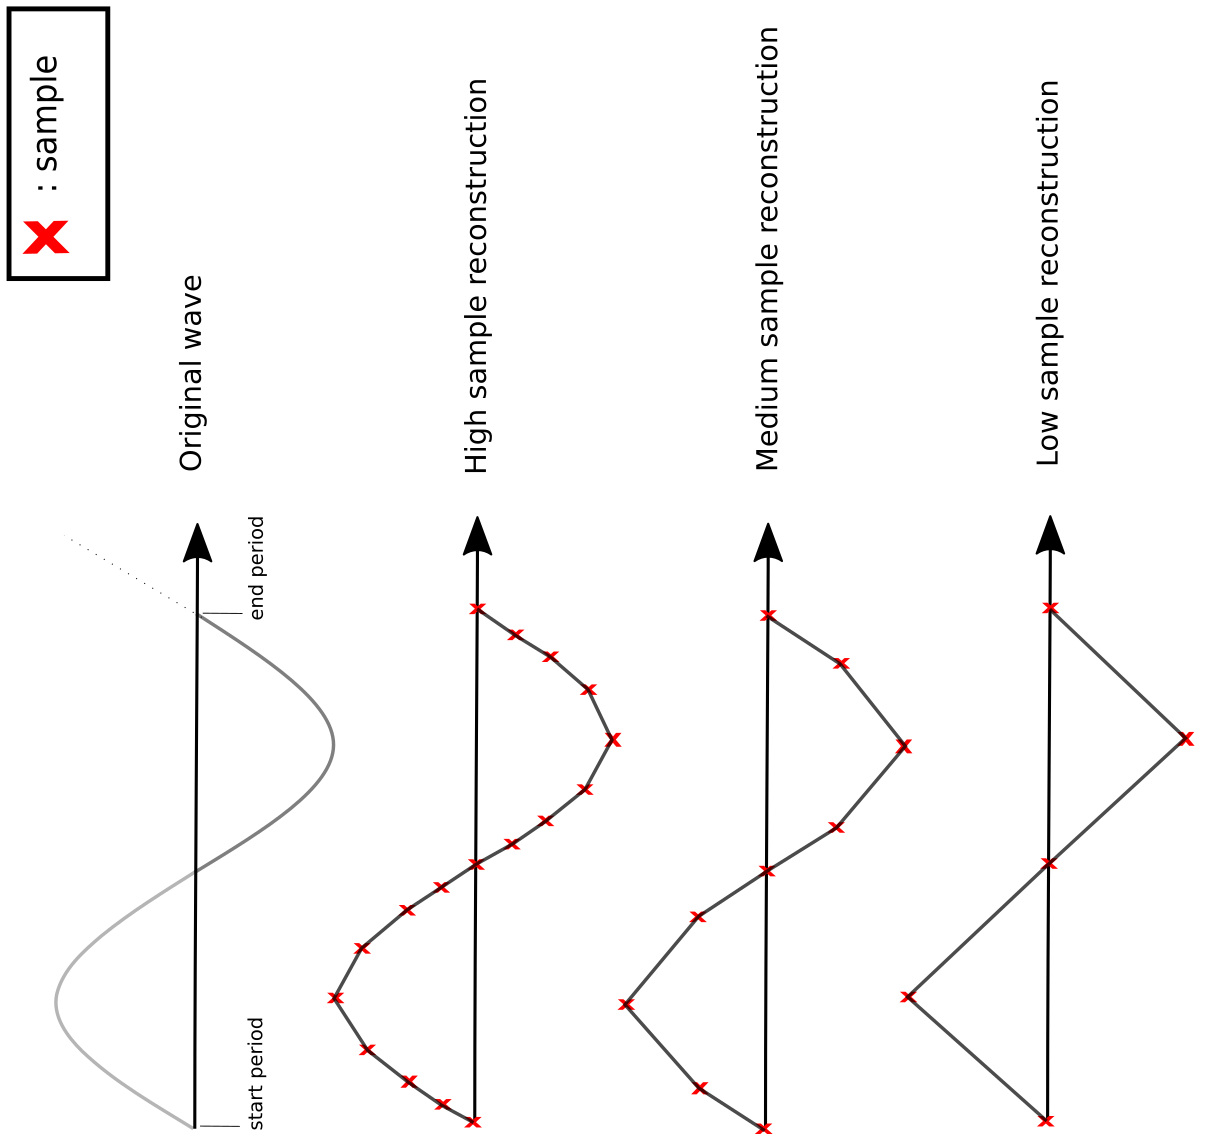
\includegraphics[width=1\linewidth,angle =-90 ]{images/periodic_function_decimation.png}
\caption{Reconstruction of signals from discrete points may result in loss of data with inadequate sampling rates. Consider the case when multiple signals with varying frequencies are overlapped.} 
\label{fig_sampling_rate}
\end{figure}


\subsection{Loudness, Amplitudes and Envelopes}
Loudness is a subjective description of a sound's intensity or energy levels. It varies based on the complexity of sounds, the frequencies present, and hearing ability of the listener~\cite{fletcher1933loudness,cook1999chap6}. It can only be measured relatively, by establishing a benchmark sound and surveying populations on the relative intensities~\cite{cook1999chap6}. Since loudness and intensity of sound correlate with the amplitude of digital waveforms (the values assigned to the samples), an imperfect but convenient alternative method for inferring the the loudness of digital sounds is to compare relative amplitudes. 

% The peak level of a digital sound corresponds to the sample with the highest value. This method has its benefits, but leaves out an important factor: the duration of intensity. A more commonly used method of level detection is the Root Mean Square (RMS) method, which averages the amplitude of multiple sequences.

Sounds typically vary in intensity as they unfold. This change in intensity is often described by the \enquote{envelope} of the sound, particularly in shorter samples. For digital sounds, Mitchell describes the envelope as either (since samples typically take the range of -1 to 1) of the borders that are created by graphing a signal and connecting the local absolute peak values~\cite{mitchell2009basicsynthChap6}. The envelope is generally described via 4 features: Attack, Decay, Sustain and Release (ADSR). Attack describes how quickly the peak loudness is reached. Decay for how quickly the sound drops to sustain level. Sustain is the duration of sustaining intensity (e.g how long a finger is kept on a piano key). Release describes the speed of fading to silence (e.g once a piano key is released).

Envelopes can be mathematically described and used to shape signals. A common approach in digital sound synthesis is to output all samples at a consistent amplitude and apply an envelope later down the synthesis chain. Digital and analog synthesizers often have built-in ADSR modules to shape the volume of the output and other parameters.  

% [Graph of envelope shaping a signal]
% note: make sure you're using terms signal and waveform properly
\subsection{Frequency, Pitch and Spectrograms}
\textit{Frequency} is used to describe number of repetitions within a time-frame, or how frequently a cycle is repeated. The frequency of an audio signal is often measured in unit of hertz (cycles per second). Most sounds, particularly those from none virtual sources, are a combination of multiple different pressure waves with different frequencies and amplitudes. \textit{Pitch}, is a perceptual property of sound that is tied to the frequencies present in each sound. How we perceive and describe the pitch of a sound (e.g high-pitched vs low-pitched) is heavily dependent on the characteristics (frequency, amplitude, duration, etc) of the waveforms it contains. Some sounds such as piano chords or pure tones have easily discernible pitches. Others, such as \enquote{pink noise} or the sound of rain do not. Yet another factor to consider is the hearing ability of the subject, which varies between people based on factors such as age, environment, musical training, etc~\cite{reiss2016meta,alain2007age,newman2012grm7}. 

% We often do not have access to the time-variant systems which create sounds. If we have access to a recording of their outputs (i.e digital sound), we can make approximations about their characteristics. 
Spectrograms are graphs used to depict the duration and amplitude of frequencies present in a sound. To create spectrograms, sound must be decomposed into a set of simpler functions. A common method for the breakdown of complex, time-variant functions is the fourier transformation and its variations. One such method is the discrete fourier transformation (DFT) and its inverse, which can convert digital sound from its time domain representation (sequence of samples) to its frequency domain representation (sets of frequency ranges and their amplitude) and vice versa.\\\\

% [spectrogram figures]

% https://en.wikipedia.org/wiki/Frequency_domain#/media/File:Fourier_transform_time_and_frequency_domains_(small).gif

\section{Digital Audio Synthesis}
\label{sec_digital_synthesis}
The phenomena of sound at intensities we commonly encounter can be described as a product of a \textit{linear system} of functions~\cite{cook1999chap4}. A linear system is a system where the transformation of overlapping inputs is equal to the sum of the separately transformed inputs~\cite{lyons2004understandingChap1,cook1999chap4}. In a linear system $\mathcal{S}$ with valid inputs and outputs $x(i)$ and $y(i)$, if:

\begin{equation}
 \mathcal{S}(x(i_1)) \xrightarrow{generates} y(i_1)
\end{equation}
\begin{center}
    and
\end{center}
\begin{equation}
\mathcal{S}(x(i_2)) \xrightarrow{generates}y(i_2)
\end{equation}

The output of the system given both inputs is the sum of the individual outputs, or:
\begin{equation}
 \mathcal{S}(x(i_1)+x(i_2)) \xrightarrow{generates} y(i_1)+y(i_2) 
\end{equation}
\\
This concept has important implications digital audio creation and analysis. Simple tones can be combined to create complex sounds, and complex sounds can be broken down for easier analysis~\cite{lyons2004understandingChap1}. It also allows systems based on experiments with simple sine waves to remain relevant in complex sound domains~\cite{cook1999chap4}.

% [graph of addition of two sine waves making a complex sine wave ]
\\

Various sound synthesis techniques have been developed via the treatment of sound as a sequence of values. Linear systems are commonly used in creation of musical tones, while non-linear systems are used for introduction of distortion and noise where needed. In their taxonomy of digital synthesis techniques, Smith defines four families of algorithms: algorithms that process and modulate existing sounds (e.g granular synthesis, wavelets), spectral models that aim to create a particular spectrum of sound (e.g additive, subtractive), physical models which emulate the physics of real instruments (discussed briefly in Section ~\ref{sec_tools_disposal}) and abstract models (e.g wave shaping, Karplus-Strong) often used for adding harmonics or distortion to simple sound signals~\cite{smith1991viewpoints}. 

Synthesizers are engines of synthesis that make use of one or more of these techniques for sound generation. Selection of the appropriate synthesis methods depends not only on the expectations from a single end product, but also the features of the synthesizer itself. Whether in goal oriented tasks such as text-to-speech or in creative endeavors such as ambient-noise generation, it is often desirable to work with systems that are quick, adaptable and tractable. For example, one might desire a text-to-speech system where slight changes to input parameters can introduces slight changes to the speech patterns, utterances, voices etc. This ability to quickly modify and audition sounds becomes a necessity when the synthesizer is being used as a creative instrument of itself, rather than an emulator for existing instruments and sounds. 

In our work, we require our synthesizer to be simple and efficient, as we would like to deploy as many instances as possible (e.g when searching for particular sounds). We also value replicability as we would like to save and re-use synthesizer programs which we found interesting. Another requirement is tractability as we would like modify parameters of a program with various levels of intensity and contrast the audition results.

Having considered our requirements, we opted to mainly utilize \enquote{additive} and \enquote{subtractive} synthesis, umbrella terms for some of the most simple and common methods of digital synthesis~\cite{mitchell2009basicsynthChap1}. 
In additive synthesis, sounds are built as a sum of signals; Where signals are outputs of oscillators (periodic wave generators).  In subtractive synthesis, segments of a complex signal are removed until a desired sound is reached, often by a chain of one or more \textit{digital filters}. Digital \textit{low-pass filters} remove or reduce the amplitude of signals with frequencies lower than a given \textit{cutoff}, while \textit{high-pass} filters filter out higher than threshold frequencies. It is not uncommon for percussive sounds to have noisy, chaotic high frequency content during their short attack envelope followed by harmonic low/medium frequency content~\cite{lakatos2000common}. We hypothesize that additive synthesis will be an appropriate when precisely tuned oscillators are needed, and subtractive synthesis can be utilized for sculpting white noise to recreate chaotic, noisy segments of the spectrum. 



% \subsection{Analog Synthesizer}
% Talk about analog synthesis briefly, so the word synthesizer feels less abstract...
\subsection{Virtual Synthesizers}
5 decades ago, Mathews claimed that any sound can be recreated via a computer by high frequency sampling of pressure waves. Additionally, he added that since \enquote{a very high sampling rate is required, and, if this process is to be useful musically, programs for generating samples from the parameters of notes must be written}~\cite{mathews1963digital}. The methods of synthesis we discussed in Section~\ref{sec_digital_synthesis} are a major component of such programs. With the exception of physical synthesis, modern chips are more than capable of simultaneously running many instances of these algorithms. To further assist with their musical utility, the majority of digital synthesis systems work in tandem with programs such as Musical Instrument Digital Interface (MIDI), which can  modulating the parameters of these synthesis methods by modulating information pertaining to ADSR and other note characteristics, often in real time~\cite{moog1986midi}.  


 The rise of Digital Audio Workstations (DAW) ~\cite{leider2004digital} and Virtual Studio Technology (VST) based plug-ins~\cite{tanev2013virtual} have rapidly transformed the sonic and material landscape of music production in the recent years. Coupled with this rise in popularity is a vast array of commercial products and services dedicated to satiating the need of amateur and professional music producers for unique sounds; most commonly via audio samples: one-shot drum samples, long sustained notes (commonly referred to as pads or textures), and loops (percussive or melodic) are common deliverables. Two notable examples of these commercial services are \textit{loopmasters}\footnote{loopmasters.com} and \textit{splice.com}\footnote{splice.com}. Furthermore, VST plug-ins can emulate complex audio synthesizers and effects which some producers may find daunting or time consuming to work with from scratch. In many cases VST plug-in vendors or unaffiliated enthusiasts sell additional presets for these plugins, targeted towards producers who do not have the time or interest in creating their own. The flexibility of the VST technology allows producers to further modify these presets until their desired sound is reached.


\section{Neural Networks And Sound}
\label{bg:NN}

\subsection{Neural Networks as Synthesizers}
We defined digital synthesis as the \enquote{process of generating discrete values which approximate sound waves}. We also established that manual generation of these values at high sampling rates is near impossible; A problem which has motivated a wide variety of synthesis techniques which aim to create signals within a linear (or mostly linear) system. Recently, the exponential increase in computing power has motivated a wide range of research in probabilistic sound generation, mainly via generative neural networks. 
% deterministically, if the input parameters to the system do not change, the output of the system will remain the same \footnote{talk about noise generation methods and seeding}.

Artificial Neural networks(ANNs) map inputs to outputs via a large network of parameters. Given the right network shape and parameter weights, they can approximate a large set of functions~\cite{cybenko1989approximation,cardaliaguet1992approximation}. ANNs are often deployed when we do not have access to the system of functions which guide a process, but a mapped set of inputs and the corresponding outputs are available. Given this set, the parameters of a neural network can be tuned for approximating the effect of the system on any valid input. The shape of the neural network (e.g number of layers, connections, activation functions) is often selected via trial and error ~\cite{bergstra2012random,bergstra2011algorithms,ba2013adaptive}. By definition, these approximations will never be more accurate than the system that is being approximated. 

Since their emergence in the 1950's, research on ANNs has gone through several eras of stunted growth~\cite{basheer2000artificial,anderson1988neurocomputing}.  In the last decade, the increase in the affordability of high performance graphic cards has been coupled with a major resurgence of interest for ANNs. As a result, a number of domain specific variations of the traditional ANN architectures have emerged. 

Generative neural networks (GNNs) are utilized for the completion of a sequences of values; Often by taking an incomplete sequence as input and outputting the most likely value for the next step. WaveNet is considered a seminal breakthrough in the usage ANNs for sound synthesis~\cite{oord2016wavenet}. Surpassing state of the art speech synthesis techniques, which create outputs with the the combination of previously recorded audio snippets~\cite{schwarz2007corpus}. When trained on a large corpus of audio samples, GNNs such WaveNet can learn the \enquote{predictive distribution for each
audio sample conditioned on all previous ones}~\cite{oord2016wavenet}. Once this distribution is learned, it can be used to create sounds 1 sample at a time, a slow process, as Mathews predicted~\cite{mathews1963digital}. \\
% Parallel WaveGAN has only 1.44 M parameters and can generate 24 kHz speech waveform 28.68 times faster than real-time on a single GPU environment. Perceptual listening test results verify that our proposed method achieves 4.16 mean opinion score within a Transformer-based text-to-speech framework, which is comparative to the best distillation-based Parallel WaveNet system.
\section{Our Synthesis Method}
 Rather than directly using neural networks for sound synthesis, we generate programs for this virtual synthesizer. Our decision is based on the following factors:
\begin{enumerate}[label=(\roman*)]
    \item \textit{Novelty and Creativity}: The goal here is to work with the limitations of any tractable sound source to create its approximations of a given sound category. We seek to create novel sounds via artificial, exploratory creativity. Boden defines this concept as an emergent property of generative work within confined rule sets~\cite{boden2009computer}. An example is the perpetual popularity of 8-bit aesthetics~\cite{collins2007loop}. 
    \item \textit{Interpretability}: Neural networks are often described as black boxes with uninterruptible weights~\cite{basheer2000artificial}. Their highly recursive structure makes modern explanation methods such as saliency maps unreliable~\cite{rudin2019stop}.  
    \item \textit{Speed of Rendering}: Neural network synthesis is costly; Sub 24 khz sample rates are common in most relevant works~\cite{yamamoto2020parallel,oord2017parallel,aouameur2019neural,ramires2020neural}. This is far below CD quality sampling rates~\cite{reiss2016meta}. At our fixed sampling rate of 48 khz, synthesizers with 8 submodules can create and save 1 second sounds to hard-disk with an average rendering time of 50 milliseconds\footnote{Using a single process on a Macbook Air 2012 and Ubuntu 18.04}. 
    \item \textit{Flexibility and Scaling}: Probabilistic audio generation is often done sequentially. State of the art, parallel wave generation with GANs requires a fixed amount of rendering time for each time-step~\cite{yamamoto2020parallel}. With our virtual synthesizer, the added footprint of increasing the length of rendered sounds or higher sampling rates is relatively minuscule.  
\end{enumerate}

\section{Goal Oriented Novel Sound Generation}

\label{related}
\subsection{Tool Selection}
We define \enquote{goal oriented novel sound generation} as any work that seeks to implement a system that is capable of generating novel sounds with a desired characteristic. Based on our review of relevant works, we believe that \enquote{goal oriented audio generation} necessitates two essential components: A tool-set for the analysis of sound and a tool-set for creation of sound. As a result, we base our work around learning of the distinguishing features of various sound groups (i.e different types of drums) and using the learned features for generation of sound. In Section~\ref{sec_methodology} we introduced these components as the virtual ear and virtual synthesizer. 

 Thus far we have discussed various techniques at our disposal for the implementation of a virtual ear and synthesizers, all with their contextual strengths and weaknesses. In the upcoming Sections, we will thoroughly discuss our implementations and the subsequent results. Here, we will review a variety of works which fall under our definition of \enquote{goal oriented novel sound generation}. Particularly, we are interested in a discussion of goals, chosen methods for the feature extraction, and chosen methods of sound synthesis. 

\subsection{Related Works}
ANN or DSP approaches can be taken to the implementation of a virtual ear and a virtual synthesizer. The development of ANN frameworks has led to works which have utilized ANNs for both components. Also common are works which have leveraged a mixture of both approaches, commonly by utilization of ANNs for the virtual ear and DSP methods for synthesis.

\begin{center}
\begin{table}[h*]
\hline
 \resizebox{\linewidth}{!}{\begin{tabular}{||c c c c||} 
work & feature extraction & synthesis & specilization & \hline
Oord et al & CNN & CNN &Speech& \hline
Yamamoto et al & GAN & GAN&Speech & \hline
Aouameur et al & Latent layer& Decoding of Latent Layers & Percussion & \hline
Ramires et al & Latent layer & FeedForward Network & Percussion & \hline
Yee-King et al & LSTM on Paremters & DSP & Synth Pads & \hline
\end{tabular}}
\caption{Quick reference for related works}
\end{table}
\end{center}
Numerous deep, neural network models have been proposed and utilized for the purpose of signal generation in recent years. WaveGans and WaveNet have been subject to significant improvements and experiments since their proposal~\cite{nsynth2017,yamamoto2020parallel,oord2017parallel}. Most relevant to us are recent works by Aoumaeur et al. in which variational AutoEncoders (VAE's) have been utilized for generation of percussive samples~\cite{aouameur2019neural}; As well as Ramires et al's work in generation of percussive sounds by guiding the output of a feedforward neural network via a small set of latent features. 
Automatic programming of virtual synthesizers has also been a topic of interest. Genetic Algorithms have long been utilized for the generation of new sounds with various sound-engines~\cite{johnson1999exploring,dahlstedt2001creating,hornermachinetongues,macret2012automatic}. More recent work by Yee-King et al.~\cite{yee2018automatic} used Long short-Term Memory (LSTM) models and genetic algorithms to find the exact parameters used to create a group of sounds. The sounds approximated were made by the same virtual synthesizer, not an external source; making the eventual replication certain even with random search. Since this work appears more focused on pads and textures rather than drums, feature matching appears to not be concerned with the envelope of the sounds but rather the frequency content within arbitrary time windows. Yet another recent work by Esling et al. used a large dataset of over 10,000 presets for a commercial VST synthesizer to learn a latent parameter space which can be sampled for creation of new audio~\cite{esling2019universal}. As stated before, our work explores the rapid approximation of percussion sounds with no previous knowledge about the sonic capabilities of our virtual synthesizer, exploring the actual parameter space rather than its latent representation.

 

\end{document}